\addtocontents{toc}{\vspace{2em}}
\chapter{Σχεδιασμός του συστήματος} % Main chapter title

\label{Chapter6} 

\section{Εισαγωγή}
Στο κεφάλαιο αυτό θα γίνει μία περιγραφή του σχεδιασμού του συστήματος ελέγχου του κάθε σιλό του LPPS ξεχωριστά. Για να γίνει αυτό και το κάθε σιλό να είναι σε θέση να αναβαθμιστεί χρησιμοποιώντας τεχνολογίες ΙοΤ είναι απαραίτητη η ενσωμάτωση ενός μικροϋπολογιστή με δυνατότητες δικτύωσης σε κάθε σιλό. Από εδώ και στο εξής ένα τέτοιο σύστημα, δηλαδή τα μηχανικά στοιχεία ενός σιλό σε συνεργασία με τον μικροϋπολογιστή, θα καλείται Industrial Automation Thing (IAT). 

	Αυτοί οι μικροϋπολογιστές, αποτελούν τους LwM2M clients του συστήματος και θα παρέχουν υπηρεσίες στο περιβάλλον τους που μπορεί να τις αξιοποιήσει ένας LwM2M server ώστε να επιτυγχάνεται η παραγωγή liqueur που είναι και το ζητούμενο. 
	
Για τον σχεδιασμό του συστήματος χρησιμοποιήθηκε η γλώσσα UML, που είναι μια γλώσσα γενικής χρήσης, ανάπτυξης και μοντελοποίησης στον τομέα της μηχανικής λογισμικού και παρέχει έναν τυποποιημένο τρόπο απεικόνισης του σχεδιασμού ενός συστήματος. Η υλοποίηση των διαγραμμάτων UML έγινε με την βοήθεια του εργαλείου Papyrus. 
	
\section{Σχεδιασμός του API του Industrial Automation Thing}

Για να γίνει ο σχεδιασμός του API του ΙΑΤ έπρεπε αρχικά να ληφθούν υπόψιν όλα τα κρίσιμα τμήματα των διεργασιών που μπορεί να εκτελέσει ένα σιλό. Τα κρίσιμα τμήματα που σημειώθηκαν και σύμφωνα με τα οποία έγινε ο σχεδιασμός του συστήματος είναι τα παρακάτω: 

\begin{itemize}
	\item{Όταν ένα σιλό γεμίζει με υγρό πρέπει οι πάνω βαλβίδα να κλείσει αμέσως μόλις ανιχνευθεί υγρό. Αν δεν γίνει αυτό το σιλό μπορεί να συνεχίζει να γεμίζει πέρα από το επιθυμητό επίπεδο. }
	\item{Όταν ένα σιλό αδειάζει από υγρό η κάτω βαλβίδα πρέπει να κλείσει αμέσως μόλις ο κάτω αισθητήρας του σιλό ανιχνεύσει απουσία υγρού. }
	\item{Όταν ένα σιλό θερμανθεί μέχρι μία συγκεκριμένη θερμοκρασία τότε το στοιχείο θέρμανσης του σιλό πρέπει να απενεργοποιηθεί άμεσα ώστε να μην ξεπεραστεί η θερμοκρασία αυτή.}
	\item{Όταν ένα σιλό έχει αναδευτεί για το επιθυμητό χρονικό διάστημα το στοιχείο μίξης πρέπει να απενεργοποιηθεί αλλιώς μπορεί να μην έχουμε το επιθυμητό αποτέλεσμα στον τελικό προϊόν.}
\end{itemize}


	Παρατηρείται ότι οι κρίσιμες λειτουργίες αφορούν τα μηχανικά στοιχεία και τις λειτουργίες μόνο ενός σιλό και έτσι δεν χρειάζεται επιπλέον γνώση οποιασδήποτε πληροφορίας ή αλληλεπίδρασης με το περιβάλλον του. Αυτό σε συνδυασμό με την παραδοχή ότι το κάθε σιλό βρίσκεται σε μεγάλη απόσταση από τα υπόλοιπα καθιστά σαφές ότι θα πρέπει να υπάρχει ενσωματωμένος ένας μικροϋπολογιστής σε κάθε σιλό ξεχωριστά και ότι το κάθε σιλό θα αποτελεί και έναν LwM2M client. Έτσι σύμφωνα με τις προδιαγραφές του OMA LwM2M ορίστηκαν κάποια συγκεκριμένα LwM2M objects καθώς και resources, μέσω των οποίων γίνεται η πρόσβαση στις υπηρεσίες που παρέχει το κάθε σιλό. Αυτά αναλύονται καλύτερα στην επόμενη ενότητα.
	
\section{Περιγραφή των LwM2M objects και resources}
Παρακάτω αναφέρονται και περιγράφονται τα LwM2M objects που ορίστηκαν για την ανάπτυξη του συστήματος ελέγχου του κάθε σιλό: 

\begin{itemize}
	\item{Object \textbf{Silo}: παρέχει τις υψηλού επιπέδου υπηρεσίες του κάθε 
	σιλό
	\begin{itemize}
		\item{Resource \textbf{state}: αναπαριστά ανά πάσα στιγμή την κατάσταση στην οποία βρίσκεται κάθε σιλό. Η κατάσταση ενός σιλό μπορεί να είναι {Empty, Emptying, Filling, Full, Heating, Heated, Mixing, Mixed}. }
		\item{Resource \textbf{initialize}: χρησιμοποιείται για διάφορες αρχικοποιήσεις που μπορεί να χρειαστεί το σιλό.}
		\item{Resource \textbf{fill}: μέσω αυτού δίνεται η εντολή για να ξεκινήσει η διαδικασία γεμίσματος του σιλό.}
		\item{Resource \textbf{empty}: μέσω αυτού δίνεται η εντολή για να ξεκινήσει η διαδικασία αδειάσματος του σιλό.}
		\item{Resource \textbf{heat}: μέσω αυτού δίνεται η εντολή για να ξεκινήσει η διαδικασία θέρμανσης του υγρού που υπάρχει στο σιλό. }
		\item{Resource \textbf{mix}: μέσω αυτού δίνεται η εντολή για να αρχίσει η διαδικασία ανάδευσης του υγρού. }
		\item{Resource \textbf{stop\_filling}: χρησιμοποιείται για να σταματήσει τη διαδικασία γεμίσματος του σιλό χωρίς αυτό να έχει γεμίσει μέχρι το μέγιστο σημείο.}
		\item{Resource \textbf{stop\_emptying}: χρησιμοποιείται για να σταματήσει η διαδικασία αδειάσματος του σιλό προτού το υγρό φτάσει στο χαμηλότερο επίπεδο του σιλό. }
		\item{Resources \textbf{filling\_completed, emptying\_completed. mixing\_completed, \\heating\_completed}: Μέσω αυτών ενημερώνεται οποιοσδήποτε ενδιαφερόμενος σχετικά με το πέρας μίας λειτουργίας. Ο κάθε ενδιαφερόμενος θα πρέπει να εγκαθιδρύσει μία σχέση observe-notify με το αντίστοιχο resource και θα λαμβάνει true κάθε φορά που μία διαδικασία του σιλό ολοκληρώνεται.}
		\item{Resource \textbf{target\_temperature}: χρησιμοποιείται για να οριστεί η θερμοκρασία μέχρι την οποία πρέπει να θερμανθεί το υγρό. Μόλις το θερμόμετρο ανιχνεύσει αυτή την θερμοκρασία τότε το υγρό σταματά να θερμαίνεται.}
		\item{Resource \textbf{event}: είναι ένα json string που περιέχει πληροφορίες για κάθε event του σιλό. Τέτοιες πληροφορίες είναι ο αποστολέας, το event (Fill, Empty, Heat, κ.ο.κ) καθώς και η ημερομηνία και η ώρα της αποστολής.}
	\end{itemize}
	}
	\item{Object \textbf{Valve}: παρέχει πρόσβαση σε υπηρεσίες χαμηλού επιπέδου μία βαλβίδας ροής υγρού.
	\begin{itemize}
		\item{Resource \textbf{on/off}: Όταν έχει την τιμή true τότε η βαλβίδα ροής υγρού είναι ανοιχτή, ειδάλλως είναι κλειστή. }
	\end{itemize}		
	}
	\item{Object \textbf{Heater}: αναφέρεται στο στοιχείο θέρμανσης του σιλό.
		\begin{itemize}
			\item{Resource \textbf{on/off}: Όταν έχει την τιμή true τότε η το υγρό θερμαίνεται, ειδάλλως το στοιχείο θέρμανσης είναι κλειστό.}
		\end{itemize}			
	}
	\item{Object \textbf{Mixer}: αναφέρεται στο στοιχείο μίξης του σιλό.
		\begin{itemize}
			\item{Resource \textbf{time to operate}: Ορίζει τον χρόνο που πρέπει να αναδευτεί το υγρό.}
			\item{Resource \textbf{on/off}: Όταν έχει την τιμή true τότε το στοιχείο μίξης είναι ενεργό, ενώ αν έχει την τιμή false το στοιχείο μίξης δεν λειτουργεί.}
		\end{itemize}			
	}
	\item{Object \textbf{Level Sensor}: παρέχει πρόσβαση σε υπηρεσίες που παρέχει ένας ανιχνευτής παρουσίας υγρού.
		\begin{itemize}
			\item{Resource \textbf{sensor type}: επιστρέφει τον τύπο του αισθητήρα.}
			\item{Resource \textbf{digital output state}: Γίνεται true όταν ανιχνευθεί υγρό από τον αισθητήρα αλλιώς είναι false.}
		\end{itemize}		
	}
\end{itemize}

	Τα LwM2M objects και resources που ορίσαμε φαίνονται πιο αναλυτικά και στον πίκανα 6.1. Αξίζει να σημειωθεί ότι μερικά από τα resources, όπως για παράδειγμα τα on/off resources υπάρχουν στο resource registry του ΟΜΑ LwM2M. Αυτά τα resources φαίνονται στον πίνακα 6.1 στα πράσινα πεδία.

\begin{table}[h]
\centering
\resizebox{\textwidth}{!}{%
\begin{tabular}{|c|c|c|c|c|c|c|c|}
\hline
\textbf{ID} & \textbf{Object} & \textbf{Resource} & \textbf{Resource	ID} & \textbf{RWE} & \textbf{Single} & \textbf{Mandatory} & \textbf{Type} \\ \hline
 &  &  &  &  & N & Y &  \\ \cline{3-8} 
 &  & state & 0 & R & Y & Y & String \\ \cline{3-8} 
 &  & initialize & 1 & E & Y & Y & Boolean \\ \cline{3-8} 
 &  & fill & 2 & E & Y & Y & Boolean \\ \cline{3-8} 
 &  & empty & 3 & E & Y & Y & Boolean \\ \cline{3-8} 
 &  & heat & 4 & E & Y & Y & Boolean \\ \cline{3-8} 
 &  & mix & 5 & E & Y & Y & Boolean \\ \cline{3-8} 
 &  & stop\_filling & 6 & E & Y & Y & Boolean \\ \cline{3-8} 
 &  & stop\_emptying & 7 & E & Y & Y & Boolean \\ \cline{3-8} 
 &  & \begin{tabular}[c]{@{}c@{}}filling\\ 			completed\end{tabular} & 10 & R & Y & Y & Boolean \\ \cline{3-8} 
 &  & \begin{tabular}[c]{@{}c@{}}emptying\\ 			completed\end{tabular} & 11 & R & Y & Y & Boolean \\ \cline{3-8} 
 &  & \begin{tabular}[c]{@{}c@{}}heating\\ 			\\ 			\\ 			completed\end{tabular} & 12 & R & Y & N & Boolean \\ \cline{3-8} 
 &  & \begin{tabular}[c]{@{}c@{}}mixing\\ 			completed\end{tabular} & 13 & R & Y & N & Boolean \\ \cline{3-8} 
 &  & \begin{tabular}[c]{@{}c@{}}target\\ 			temperature\end{tabular} & 14 & RW & Y & N & Float \\ \cline{3-8} 
\multirow{-15}{*}{20000} & \multirow{-15}{*}{Silo} & Event & 15 & R & Y & Y & String \\ \hline
\multicolumn{1}{|l|}{} &  &  &  &  & N & N &  \\ \cline{3-8} 
\multicolumn{1}{|l|}{\multirow{-2}{*}{20001}} & \multirow{-2}{*}{Valve} & \cellcolor[HTML]{32CB00}on/off & \cellcolor[HTML]{32CB00}5850 & \cellcolor[HTML]{32CB00}RW & \cellcolor[HTML]{32CB00}Y & \cellcolor[HTML]{32CB00}Y & \cellcolor[HTML]{32CB00}Boolean \\ \hline
\multicolumn{1}{|l|}{} &  &  &  &  & N & N &  \\ \cline{3-8} 
\multicolumn{1}{|l|}{} &  & \cellcolor[HTML]{32CB00}\begin{tabular}[c]{@{}c@{}}sensor\\ 			type\end{tabular} & \cellcolor[HTML]{32CB00}5751 & \cellcolor[HTML]{32CB00}R & \cellcolor[HTML]{32CB00}Y & \cellcolor[HTML]{32CB00}N & \cellcolor[HTML]{32CB00}String \\ \cline{3-8} 
\multicolumn{1}{|l|}{\multirow{-3}{*}{20002}} & \multirow{-3}{*}{Level Sensor} & \cellcolor[HTML]{32CB00}\begin{tabular}[c]{@{}c@{}}digital\\ 			output state\end{tabular} & \cellcolor[HTML]{32CB00}5550 & \cellcolor[HTML]{32CB00}RW & \cellcolor[HTML]{32CB00}Y & \cellcolor[HTML]{32CB00}Y & \cellcolor[HTML]{32CB00}Boolean \\ \hline
 &  &  &  &  & N & N &  \\ \cline{3-8} 
 &  & \begin{tabular}[c]{@{}c@{}}time\\ 			to operate\end{tabular} & 0 & RW & Y & Y & Integer \\ \cline{3-8} 
\multirow{-3}{*}{20004} & \multirow{-3}{*}{Mixer} & \cellcolor[HTML]{32CB00}on/off & \cellcolor[HTML]{32CB00}5850 & \cellcolor[HTML]{32CB00}RW & \cellcolor[HTML]{32CB00}Y & \cellcolor[HTML]{32CB00}Y & \cellcolor[HTML]{32CB00}Boolean \\ \hline
 &  &  &  &  & N & N &  \\ \cline{3-8} 
\multirow{-2}{*}{20005} & \multirow{-2}{*}{Heater} & \cellcolor[HTML]{32CB00}on/off & \cellcolor[HTML]{32CB00}5850 & \cellcolor[HTML]{32CB00}RW & \cellcolor[HTML]{32CB00}Y & \cellcolor[HTML]{32CB00}Y & \cellcolor[HTML]{32CB00}Boolean \\ \hline
\end{tabular}%
}
\caption{LwM2M objects και Resources}
\label{my-label}
\end{table}
\newpage
\section{Αρχιτεκτονικός σχεδιασμός του συστήματος ελέγχου του σιλό}
Μια αφαιρετική περιγραφή της αρχιτεκτονικής του σιλό φαίνεται στην εικόνα 6.1. Το σιλό αποτελείται από τα μηχανικά του μέρη, που είναι όλοι οι αισθητήρες, οι βαλβίδες, το στοιχείο μίξης και το στοιχείο θέρμανσης. Αυτά τα μέρη πρέπει να επικοινωνούν με κάποιο λογισμικό ώστε να μπορούν να ελεγχθούν. Η επικοινωνία των μηχανικών στοιχείων του σιλό με το λογισμικό γίνεται μέσω του driver. Ο driver ή οι drivers με τη σειρά τους αποστέλλουν πληροφορίες στον Controller του σιλό ο οποίος αποτελεί την καρδιά του συστήματος ελέγχου και με την σειρά του μπορεί να στείλει κάποιο μήνυμα στους drivers ώστε να γίνει μία ενέργεια στα μηχανικά μέρη του σιλό. Για να ενταχθεί όμως το σύστημα αυτό στο διαδίκτυο των αντικειμένων πρέπει να υπάρχει συνδεσιμότητα με το διαδίκτυο. Αυτό γίνεται μέσω του LwM2M Wrapper ο οποίος δίνει τη δυνατότητα στο σιλό να επικοινωνεί με το δίκτυο χρησιμοποιώντας το πρωτόκολλο LwM2M. Έτσι το σιλό εντάσσεται στο διαδίκτυο των αντικειμένων και παρέχει τις υπηρεσίες του στο περιβάλλον ώστε να μπορέσουν να χρησιμοποιηθούν από έναν LwM2M server για την παραγωγή ενός τύπου liqueur. 


\begin{figure}[h]
	\centering
		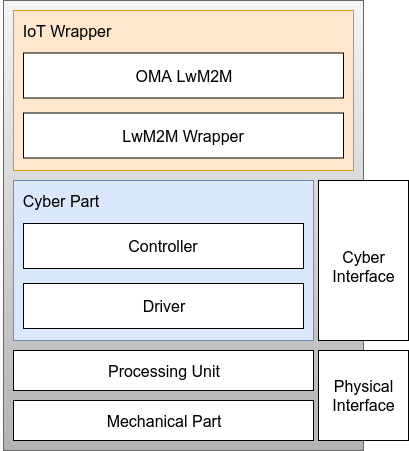
\includegraphics[height=11.5cm,width=10cm]{Figures/12.png}
	\caption{Η αρχιτεκτονική του σιλό}	
\end{figure}

	Η μεταφορά μηνυμάτων από τους drivers προς το σύστημα ελέγχου και το ανάποδο και από το δίκτυο προς το σιλό αλλά και από το σιλό προς το δίκτυο γίνεται με την χρήση Events. Στην συνέχεια θα γίνει μια εκτενέστερη αναφορά στον τρόπο που γίνεται αυτό καθ’ όλη την διάρκεια λειτουργίας του συστήματος. 
	
\section{Δομή των σιλό}

Όπως έχει ήδη αναφερθεί, στην παρούσα εργασία η ανάπτυξη του λογισμικού έγινε  βασισμένη σε συνιστώσες. Για να γίνει κάτι τέτοιο έπρεπε πρώτα να ξεχωριστούν οι διάφορες συνιστώσες από τις οποίες απαρτίζεται το σύστημα. Όπως φαίνεται και στην εικόνα 6.1 στην αρχιτεκτονική του σιλό το cyber μέρος του αποτελείται από τον driver ή τους drivers αν αυτοί είναι περισσότεροι από έναν και τον controller. Εξαιτίας αυτού έγινε η επιλογή οι διάφοροι drivers να είναι ξεχωριστά components στο σύστημα μας. Το ίδιο ισχύει και για τον controller του σιλό. Κάτι τέτοιο μας επιτρέπει να επωφεληθούμε από πολλά πλεονεκτήματα που μας δίνει τόσο αυτή η προσέγγιση όσο και το συγκεκριμένο framework (OSGi) που χρησιμοποιήσαμε, καθώς σε περίπτωση που χρειαστεί κάποια αλλαγή στο λογισμικό του συστήματος τότε αυτή μπορεί να γίνει κατά την διάρκεια που το σύστημα λειτουργεί χωρίς να επιφέρει κάποιο πρόβλημα στην λειτουργία όλου του συστήματος ελέγχου. Στις εικόνες 6.2, 6.3, 6.4, 6.5 φαίνεται η εσωτερική δομή του cyber μέρους των σιλό η οποία αποτελείται από τον controller μαζί με το state machine του που καθορίζει την συμπεριφορά του σιλό και την υποδομή των drivers του σιλό. Μέσω των διάφορων ports ο controller του σιλό επικοινωνεί με τους drivers και το περιβάλλον του.  

\begin{figure}[htbp]
	\centering
		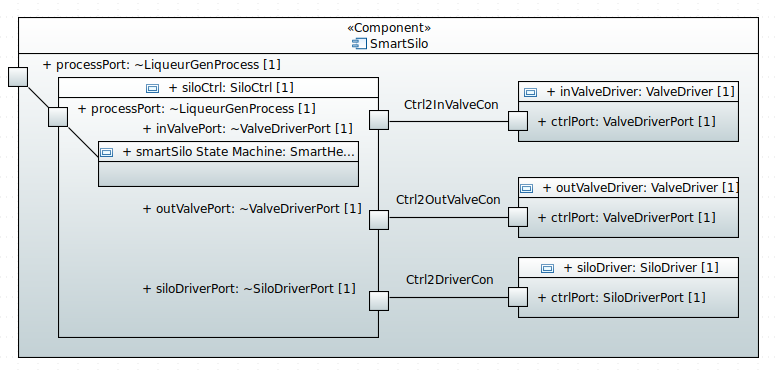
\includegraphics[height=9.5cm,width=15cm]{Figures/13.png}
	\caption{H δομή του smartSilo1}	
\end{figure}
\begin{figure}[htbp]
	\centering
		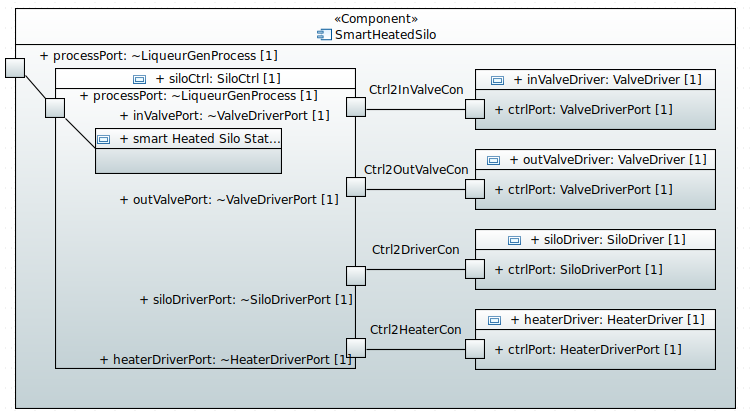
\includegraphics[height=9cm,width=15cm]{Figures/14.png}
	\caption{H δομή του smartSilo2}	
\end{figure}
\begin{figure}[htbp]
	\centering
		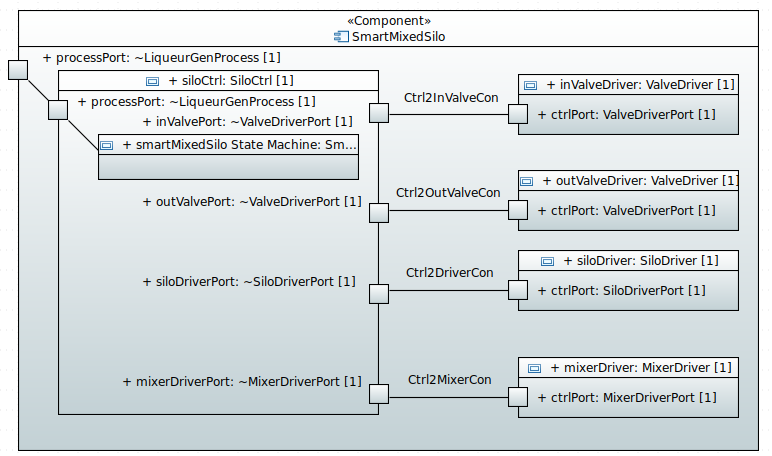
\includegraphics[height=9cm,width=15cm]{Figures/15.png}
	\caption{H δομή του smartSilo3}	
\end{figure}
\begin{figure}[htbp]
	\centering
		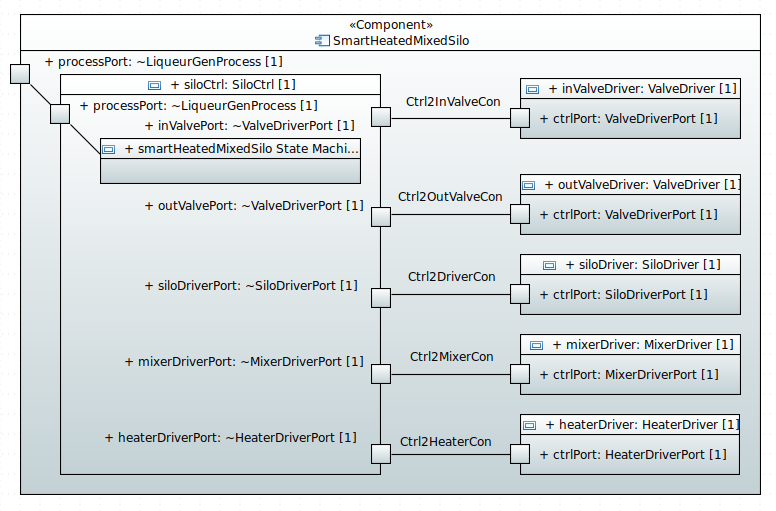
\includegraphics[height=10cm,width=15cm]{Figures/16.png}
	\caption{H δομή του smartSilo4}	
\end{figure}

\newpage

 Η δομή της συνιστώσας του controller του σιλό φαίνεται στο διάγραμμα κλάσεων της εικόνας 6.6. Η notifica-tionQueue αποτελεί την EventQueue του controller στην οποία έρχονται όλα τα μηνύματα από το περιβάλλον του σιλό. Επιπλέον μέσα από το διάγραμμα μπορούμε να ξεχωρίσουμε τις διάφορες καταστάσεις του σιλό καθώς και τον τρόπο μετάβασης από την μία μετάβαση στην άλλη μέσω των διάφορων Transitions. Παρατηρούμε επίσης ότι έχουμε ορίσει δύο κλάσεις τις State και Transition οι οποίες αποτελούν υπερκλάσεις και κληρονομούνται από τις επιμέρους καταστάσεις του σιλό και από τις μεταβάσεις από την μία κατάσταση στην άλλη αντίστοιχα. 
 
\begin{figure}[htbp]
	\centering
		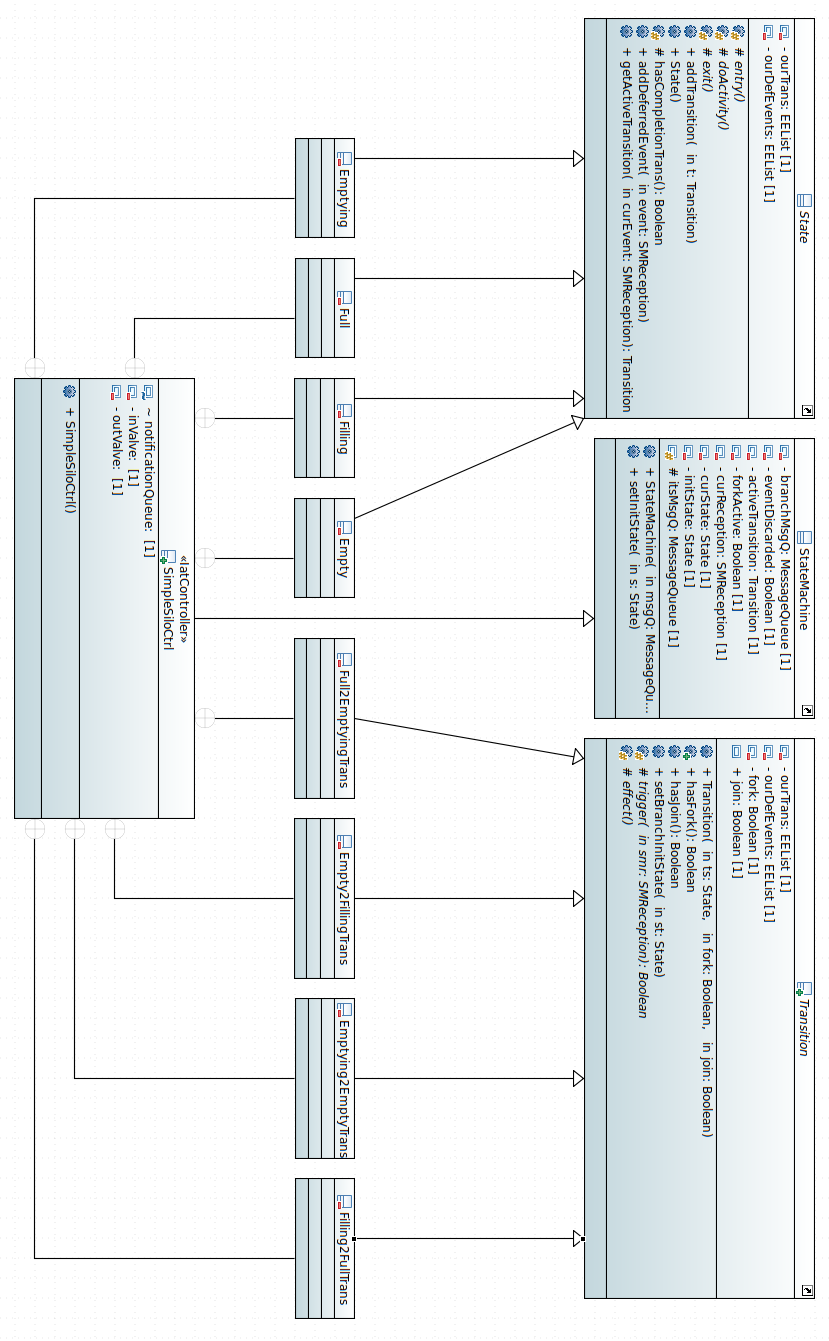
\includegraphics[height=20cm,width=14cm]{Figures/23.png}
	\caption{To διάγραμμα κλάσεων του state machine του σιλό}	
\end{figure}

\section{Συμπεριφορά του συστήματος ελέγχου}
Κάθε σιλό μπορεί να θεωρηθεί ότι κάθε στιγμή βρίσκεται σε μία συγκεκριμένη κατάσταση μέσα από ένα πεπερασμένο πλήθος καταστάσεων. Με την λήψη ενός μηνύματος είτε από τους drivers είτε από έναν LwM2M server το σιλό εκτελεί τις απαραίτητες λειτουργίες και μεταβαίνει στην επόμενη κατάσταση του. 

Ας πάρουμε για παράδειγμα, τις καταστάσεις του σιλό που περιλαμβάνει στοιχείο θέρμανσης την στιγμή που ξεκινά η λειτουργία παραγωγής liqueur τύπου Β. Αρχικά το σιλό είναι άδειο και βρίσκεται στην κατάσταση \textbf{EMPTY}. Όταν ο LwM2M client λάβει το μήνυμα Fill από τον LwM2M server τότε θα ανοίξει η πάνω βαλβίδα εισαγωγής υγρού και το σιλό θα αρχίσει να γεμίζει με liqueur και θα μεταβεί στην κατάσταση \textbf{FILLING}. Στην συνέχεια, αν ο άνω αισθητήρας ανίχνευσης υγρού ενεργοποιηθεί, δηλαδή ανιχνεύσει υγρό τότε ο driver στέλνει το μήνυμα StopFilling και το σιλό μεταβαίνει στην κατάσταση \textbf{FULL}. Ένα τέτοιο μήνυμα μπορεί να έρθει και από τον LwM2M server σε περίπτωση που κάποιος θέλει να διακόψει την εισαγωγή υγρού στο σιλό. Στην συνέχεια έρχεται από τον server ένα μήνυμα Heat και αρχίζει η λειτουργία του στοιχείου θέρμανσης του σιλό, το οποίο εισέρχεται στην κατάσταση \textbf{HEATING} μέχρις ότου φτάσει το υγρό στην επιθυμητή θερμοκρασία. Όταν γίνει αυτό ο αισθητήρας θερμοκρασίας στέλνει μέσω του driver ένα μήνυμα HeatingCompleted και το σιλό μεταβαίνει στην κατάσταση \textbf{HEATED}. Τέλος, με ένα μήνυμα Empty το σιλό μεταβαίνει στην κατάσταση \textbf{EMPTYING} και ανοίγει η βαλβίδα εξαγωγής υγρού. Μόλις το υγρό αδειάσει το σιλό μεταβαίνει στην κατάσταση \textbf{EMPTY} και η διαδικασία επαναλαμβάνεται. Αυτή η διαδικασία αναπαρίσταται από το state machine της εικόνας 6.7. Παρόμοια συμπεριφορά έχουν και τα υπόλοιπα σιλό όπως φαίνεται και στις εικόνες 6.6, 6.8, 6.9.


 Παρατηρούμε ότι όταν το σιλό βρίσκεται σε μία κατάσταση τότε πρέπει να εκτελεστεί μία λειτουργία από κάποιον driver. Όπως για παράδειγμα όταν το σιλό βρίσκεται στην κατάσταση \textbf{FILLING} ο driver πρέπει να στείλει μήνυμα στην άνω βαλβίδα ροής υγρού του σιλό ώστε αυτή να ανοίξει και όταν ο άνω αισθητήρας ανίχνευσης υγρού του σιλού ανιχνεύσει υγρό τότε η βαλβίδα πρέπει να κλείσει. Η επικοινωνία αυτή γίνεται μέσω της EventQueue του controller. Πιο αναλυτικά, όταν ο LwM2M  server που εκτελεί μια διεργασία παραγωγής liqueur ενός εκ των δύο τύπων στείλει ένα μήνυμα στον  LwM2M client του σιλό, τότε μέσω των υπηρεσίων που παρέχει η συνιστώσα του controller στο περιβάλλον της τα μηνύματα αυτά μεταφέρονται στην EventQueue του controller και από εκεί αποστέλονται τα ανάλογα μηνύματα στους drivers του σιλό μέσα από τις υπηρεσίες που η αντίστοιχη συνιστώσα του εκάστοτε driver παρέχει στο περιβάλλον της. 


\begin{figure}[htbp]
	\centering
		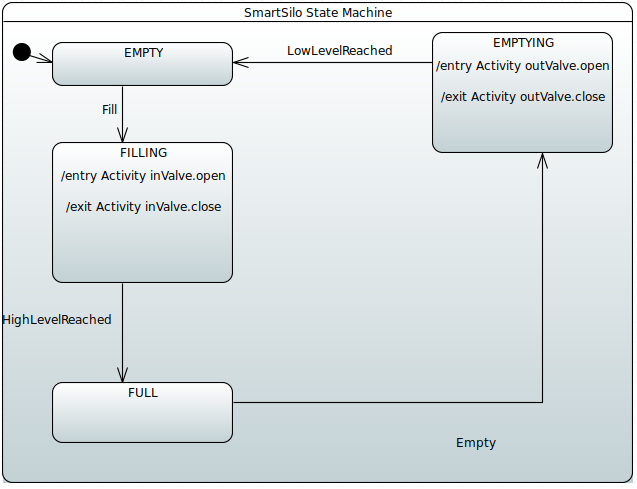
\includegraphics[height=10cm,width=15cm]{Figures/17.png}
	\caption{Το state machine του smartSilo1}	
\end{figure}
\begin{figure}[htbp]
	\centering
		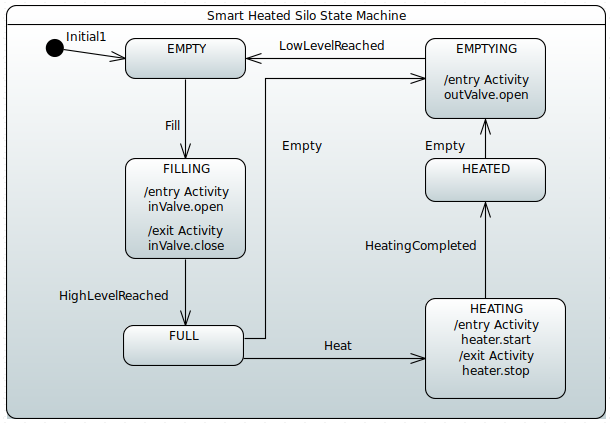
\includegraphics[height=10cm,width=15cm]{Figures/18.png}
	\caption{Το state machine του smartSilo2}	
\end{figure}
\begin{figure}[htbp]
	\centering
		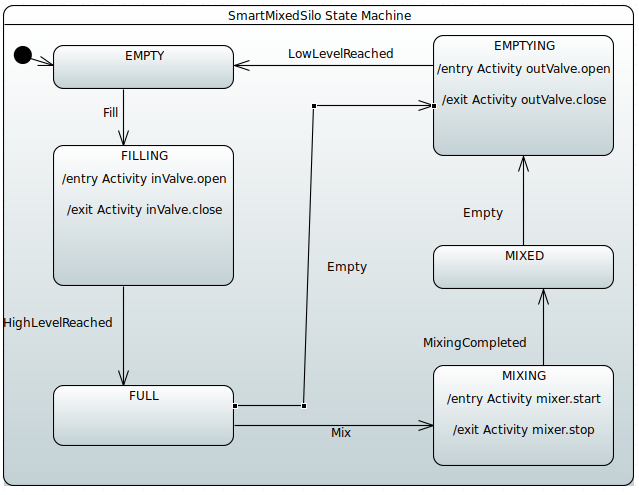
\includegraphics[height=10cm,width=15cm]{Figures/19.png}
	\caption{Το state machine του smartSilo3}	
\end{figure}
\begin{figure}[htbp]
	\centering
		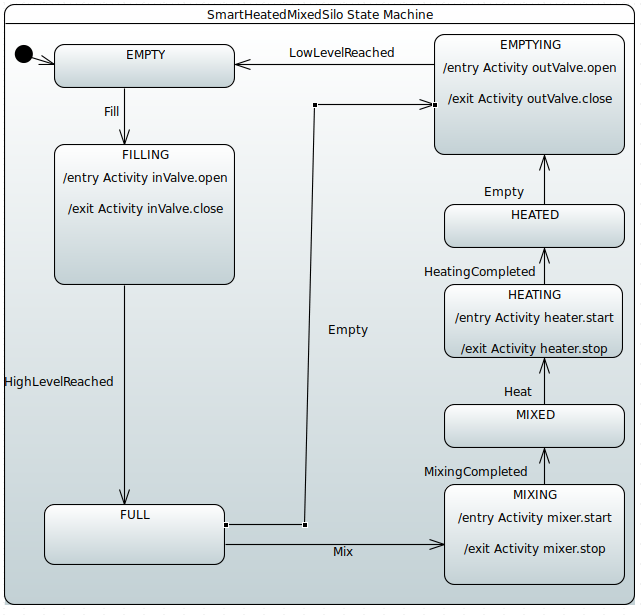
\includegraphics[height=12cm,width=15cm]{Figures/20.png}
	\caption{Το state machine του smartSilo4}	
\end{figure}




